\documentclass[letterpaper,12pt]{article}
\usepackage{array}
\usepackage{threeparttable}
\usepackage{geometry}
\geometry{letterpaper,tmargin=1in,bmargin=1in,lmargin=1.25in,rmargin=1.25in}
\usepackage{fancyhdr,lastpage}
\pagestyle{fancy}
\lhead{}
\chead{}
\rhead{}
\lfoot{}
\cfoot{}
\rfoot{\footnotesize\textsl{Page \thepage\ of \pageref{LastPage}}}
\renewcommand\headrulewidth{0pt}
\renewcommand\footrulewidth{0pt}
\usepackage[format=hang,font=normalsize,labelfont=bf]{caption}
\usepackage{listings}
\lstset{frame=single,
  language=Python,
  showstringspaces=false,
  columns=flexible,
  basicstyle={\small\ttfamily},
  numbers=none,
  breaklines=true,
  breakatwhitespace=true
  tabsize=3
}
\usepackage{amsmath}
\usepackage{amssymb}
\usepackage{amsthm}
\usepackage{harvard}
\usepackage{setspace}
\usepackage{float,color}
\usepackage[pdftex]{graphicx}
\usepackage{hyperref}
\hypersetup{colorlinks,linkcolor=red,urlcolor=blue}
\theoremstyle{definition}
\newtheorem{theorem}{Theorem}
\newtheorem{acknowledgement}[theorem]{Acknowledgement}
\newtheorem{algorithm}[theorem]{Algorithm}
\newtheorem{axiom}[theorem]{Axiom}
\newtheorem{case}[theorem]{Case}
\newtheorem{claim}[theorem]{Claim}
\newtheorem{conclusion}[theorem]{Conclusion}
\newtheorem{condition}[theorem]{Condition}
\newtheorem{conjecture}[theorem]{Conjecture}
\newtheorem{corollary}[theorem]{Corollary}
\newtheorem{criterion}[theorem]{Criterion}
\newtheorem{definition}[theorem]{Definition}
\newtheorem{derivation}{Derivation} % Number derivations on their own
\newtheorem{example}[theorem]{Example}
\newtheorem{exercise}[theorem]{Exercise}
\newtheorem{lemma}[theorem]{Lemma}
\newtheorem{notation}[theorem]{Notation}
\newtheorem{problem}[theorem]{Problem}
\newtheorem{proposition}{Proposition} % Number propositions on their own
\newtheorem{remark}[theorem]{Remark}
\newtheorem{solution}[theorem]{Solution}
\newtheorem{summary}[theorem]{Summary}
%\numberwithin{equation}{section}
\bibliographystyle{aer}
\newcommand\ve{\varepsilon}
\newcommand\boldline{\arrayrulewidth{1pt}\hline}

\setlength{\parindent}{0pt}

\begin{document}

\begin{flushleft}
  \textbf{\large{Problem Set \#1}} \\
  Reiko Laski
\end{flushleft}

\vspace{3mm}

\textbf{Exercise 1} \\
1. The state variables are the barrels of oil $B$ and the price $p_{t}$. \\
2. The control variables are $q_t$, the quantity of oil the owner choses to sell at time $t$. \\
3. The transition equation is $B_{t+1} = B_t - q_t$ \\
4. The sequence problem of the owner is
\begin{equation*}
  V(B) = \max_{q_1, q_2, \cdots} \sum_{t=0}^\infty  \Big(\frac{1}{1 + r} \Big)^t p_t q_t .
\end{equation*}
The Bellman equation is
\begin{equation*}
  V(B_t) = \max_{q_t} p_t q_t + \Big(\frac{1}{1 + r}\Big) V(B_{t+1}) .
\end{equation*}
5. The owner's Euler equation is
\begin{equation*}
  p_t = \Big(\frac{1}{1 + r}\Big) p_{t+1}.
\end{equation*}
We substitute the transition equation into the Bellman equation
\begin{equation*}
  V(B_t) = \max_{B_{t+1}} p_t (B_t - B_{t+1}) + \Big(\frac{1}{1+r}\Big) V(B_{t+1}).
\end{equation*}
The first order condition says
\begin{equation}
  \frac{dV}{d B_{t+1} } = -p_t + \frac{1}{1+r} V'(B_{t+1}) = 0
  \implies p_t = \frac{1}{1+r} V'(B_{t+1})
\end{equation}
Additionally, using the envelope condition,
\begin{equation}
  \frac{dV}{dB_t} = p_t - p_t \frac{dB_{t+1}}{dB_t} + \frac{1}{1+r} V'(B_{t+1}) \frac{dB_{t+1}}{dB_t} \implies V'(B_t) = p_t \quad \text{and} \quad V'(B_{t+1}) = p_{t+1} .
\end{equation}
Substituting (2) into (1), gives us the Euler equation. \\
6. If $p_{t+1} = p_t$ for all $t$, the owner will sell all B barrels of oil in the first period. If $p_{t+1} > (1 + r)p_t$ for all $t$, the owner will never sell any oil. The conditon on the path of prices necessary for an interior solution is $p_t < p_{t+1} < (1 + r)p_t$ .

\vspace{3mm}

\textbf{Exercise 2} \\
1. The state variables are $k_t, z_t, \text{ and } y_t$. \\
2. The control variables are $c_t$ and $i_t$.
3. The Bellman equation that represents this sequence problem is
\begin{equation*}
  V(k_t, z_t) = \max_{c} u(c_t) + \beta E[V(k_{t+1}, z_{z+1})] .
\end{equation*}

\begin{figure}[H]\centering\captionsetup{width=0in}
  \fbox{\resizebox{3.0in}{2.0in}{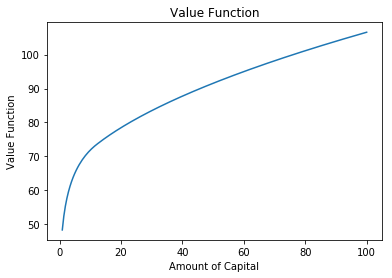
\includegraphics{ValFunc.png}}}
  \fbox{\resizebox{3.0in}{2.0in}{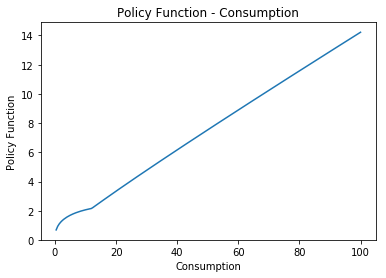
\includegraphics{PolFunc_cons.png}}}
  \fbox{\resizebox{3.0in}{2.0in}{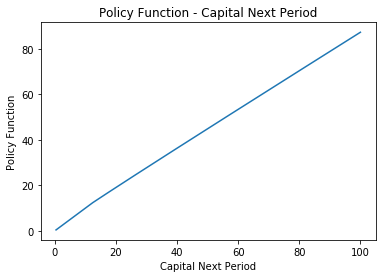
\includegraphics{PolFunc_sav.png}}}
\end{figure}

\newpage

\textbf{Exercise 3}\\
1. The Bellman equation that represents this sequence problem is
\begin{equation*}
  V(k_t, z_t) = \max_{c} u(c_t) + \beta E_{z_{t+1} | {z_t}}[V(k_{t+1}, z_{z+1})] .
\end{equation*}

\begin{figure}[H]\centering\captionsetup{width=0in}
  \fbox{\resizebox{3.0in}{2.0in}{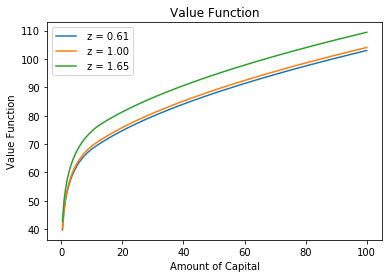
\includegraphics{ValFunc2.png}}}
  \fbox{\resizebox{3.0in}{2.0in}{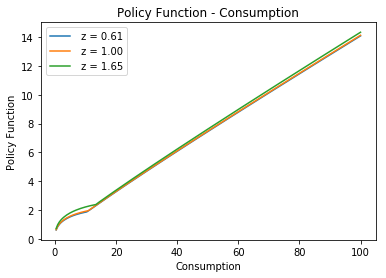
\includegraphics{PolFunc_cons2.png}}}
  \fbox{\resizebox{3.0in}{2.0in}{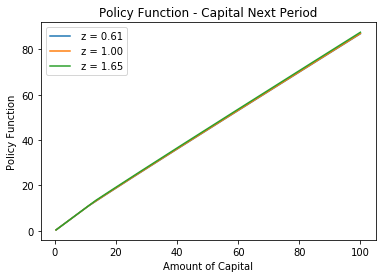
\includegraphics{PolFunc_sav2.png}}}
\end{figure}

\textbf{Exercise 4} \\
The Bellman equation representing this optimal stopping problem is
\begin{equation*}
  V(w_t) = \max\{\frac{w_t}{1-\beta}, b + \beta E[V(w_{t+1})]\} .
\end{equation*}

\begin{figure}[H]\centering\captionsetup{width=0in}
  \fbox{\resizebox{3.0in}{2.0in}{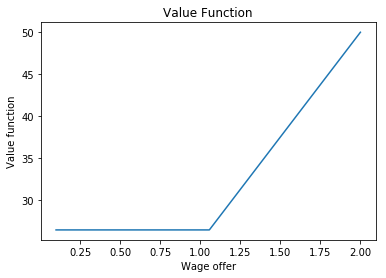
\includegraphics{ValFunc3.png}}}
\end{figure}

The reservation wage for the unemployed worker that makes her indifferent between accepting the job offer and not for $b = 0.05$ is 1.057.

\begin{figure}[H]\centering\captionsetup{width=0in}
  \fbox{\resizebox{3.0in}{2.0in}{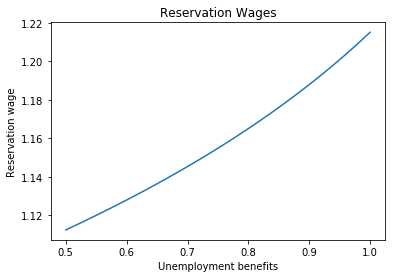
\includegraphics{ResWage.png}}}
\end{figure}

As unemployment benefits vary from 0.5 to 1.0, the reservation wage increases.

\end{document}
